\documentclass{article}
\usepackage[utf8]{inputenc}

\title{EE2703: Assignment 6L (Laplace Transform)}
\author{Yogesh Agarwala \\ EE19B130}
\date{April 18, 2021}


\usepackage{natbib}
\usepackage{graphicx}
\usepackage{amsmath}
\usepackage{listings}

\begin{document}

\maketitle

\section{Introduction}
In this assignment, we will look at how to analyze “Linear Time-invariant Systems” using the scipy.signal library in Python .We limit our analysis to systems with rational polynomial transfer functions. More specifically we consider 3 systems: A forced oscillatory system, A coupled system of Differential Equations and an RLC low pass filter  

\section{Assignment}
\subsection{Time Response of a Spring}
The goal is to obtain the time response of a spring system given by the
equation:
\begin{equation}
    \ddot x + 2.25x = f(t)
\end{equation}
We solve for $X(s)$ using the following equation, derived from the above equation.
\begin{equation}
    X(s) = \frac{F(s)}{s^2+2.25}
\end{equation}
We then use the impulse response of $X(s)$ to get its inverse Laplace transform.

\lstset{language=Python}
\lstset{frame=lines}
\lstset{label={lst:code_direct}}
\lstset{basicstyle=\footnotesize}
\begin{lstlisting}
def func_H(freq,decay):
	num = np.poly1d([1,freq])
	den = np.poly1d([1,(2*freq),((freq*freq)+(decay*decay))])
	return num, den

num,den = func_H(0.5,1.5)
den = np.polymul([1,0,2.25],den)
H1 = sp.lti(num,den)
t = np.linspace(0,50,1000)
t,x = sp.impulse(H1,T=t)
display_plot(0,t,x,"Spring with decay = 0.5", 'time','x')
\end{lstlisting}


\begin{figure}[h!]
\centering
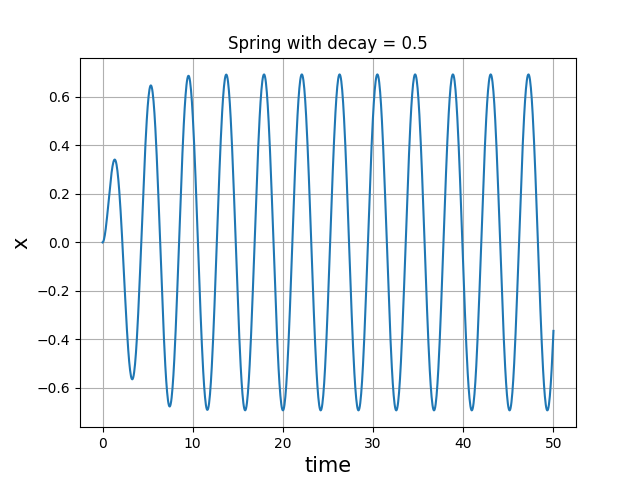
\includegraphics[scale=0.52]{Figure_0}
\caption{System Response with Decay = 0.5}
\label{fig:System Response with Decay = 0.5}
\end{figure}


\subsection{Time Response of a Spring with a much smaller decay}


\begin{lstlisting}
num,den = func_H(0.05,1.5)
den = np.polymul([1,0,2.25],den)
H2 = sp.lti(num,den)
t = np.linspace(0,50,1000)
t,x = sp.impulse(H2,T=t)
display_plot(0,t,x,"Spring with decay = 0.05", 'time','x')
\end{lstlisting}
We can notice that this time system takes longer to reach a steady state.
\begin{figure}[h!]
\centering
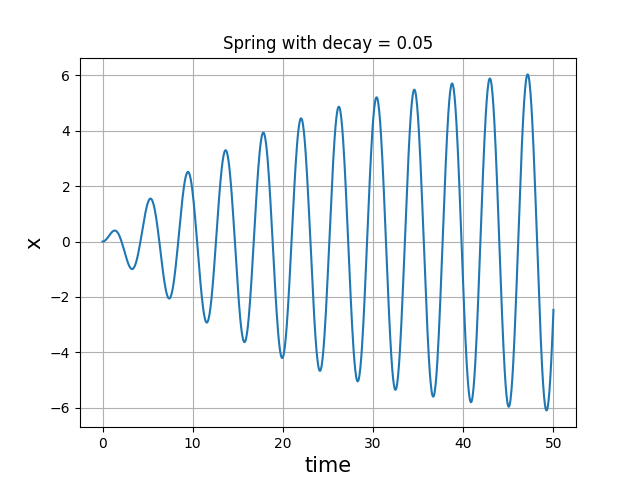
\includegraphics[scale=0.52]{Figure_1}
\caption{System Response with Decay = 0.05}
\label{fig:System Response with Decay = 0.05}
\end{figure}


\subsection{LTI response over different frequencies of applied force}
We now see what happens when we vary the frequency.
We note the the amplitude is maximum at frequency = 1.5, which is the natural frequency of the given system
\begin{lstlisting}
freqs = np.linspace(1.4,1.6,5)
leg = []
for freq in freqs:
	num = np.poly1d([1]) # Numerator of transfer function
	den = np.poly1d([1,0,2.25]) # Denominator of tranfer functioin
	H = sp.lti(num,den) # Transfer function
	t = np.linspace(0,150,5001) # Time range for graph
	f = np.cos(freq*t)*np.exp(-0.05*t) # Forcing function
	t,y,svec=sp.lsim(H,f,t) # Output wave found as convolution
	leg.append("freq =" + str(freq))
	pylab.xlabel('time')
	pylab.ylabel('X')
	pylab.plot(t,y)	
pylab.grid()
pylab.legend(leg)
pylab.show()
\end{lstlisting}

\begin{figure}[h!]
\centering
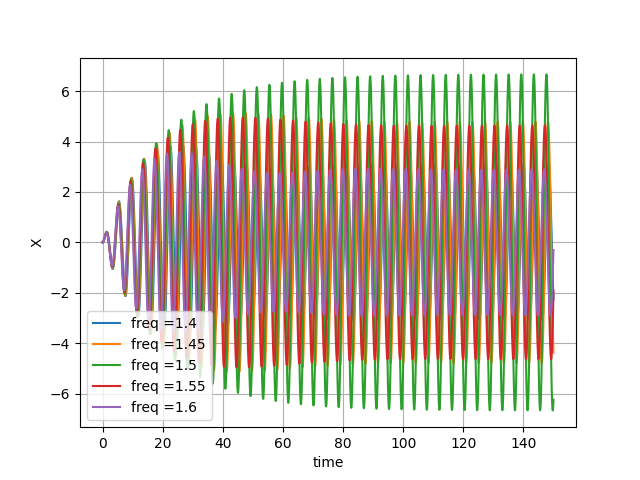
\includegraphics[scale=0.6]{Figure_2}
\caption{System Response over different frequencies}
\label{fig:System Response over different frequencies}
\end{figure}


\clearpage
\subsection{Coupled Spring System}
We now consider a coupled Differential system
\begin{equation}
    \ddot x + (x-y) = 0
\end{equation}
and 
\begin{equation}
    \ddot y + 2(y-x) = 0
\end{equation}

with the initial conditions: $\dot x(0) =0,\dot y(0) =0,x(0) =1,y(0) =0$.
Taking Laplace Transform and solving for $X(s)$ and $Y(s)$, We get:
\begin{equation}
    X(s) = \frac{s^2+2}{s^3 + 3s}
\end{equation}
\begin{equation}
    Y(s) = \frac{2}{s^3 + 3s}
\end{equation}
\begin{lstlisting}
Hx = sp.lti(np.poly1d([1,0,2]),np.poly1d([1,0,3,0]))
t = np.linspace(0,20,1000)
t1,x = sp.impulse(Hx,T=t)
pylab.plot(t1,x)

Hy = sp.lti(np.poly1d([2]),np.poly1d([1,0,3,0]))
t = np.linspace(0,20,1000)
t2,y = sp.impulse(Hy,T=t)
pylab.plot(t2,y)
\end{lstlisting}
We notice that the outputs of this system are 2 sinusoids which are out of phase.This system can be realized by creating an undamped single spring double mass system.
\begin{figure}[h!]
\centering
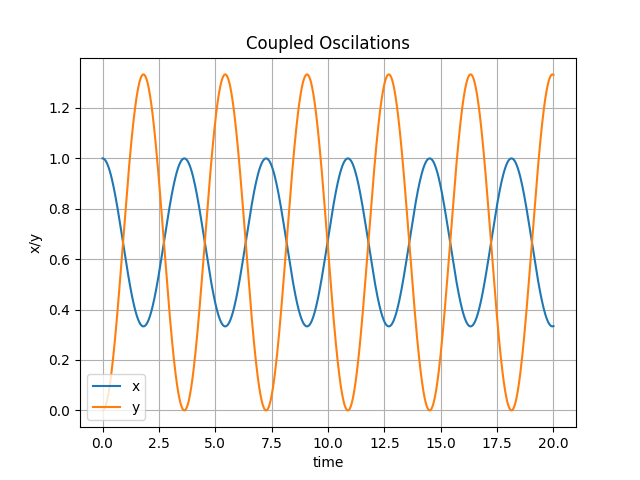
\includegraphics[scale=0.55]{Figure_3}
\caption{Coupled Oscillations}
\label{fig:Coupled Oscillations}
\end{figure}
\clearpage
\subsection{Magnitude and Phase response of Two port network}

Now we try to create the bode plots for the low pass filter defined in the question
\begin{lstlisting}
H = sp.lti(np.poly1d([1000000]),np.poly1d([0.000001,100,1000000]))
w,S,phi=H.bode()
"""
Magnitude response
"""
pylab.subplot(2,1,1)
pylab.semilogx(w,S)
pylab.ylabel(r'$|H(s)|$')
pylab.grid()
"""
Phase response
"""
pylab.subplot(2,1,2)
pylab.semilogx(w,phi)
pylab.ylabel(r'$\angle(H(s))$')
pylab.grid()
pylab.show()
\end{lstlisting}

\begin{figure}[h!]
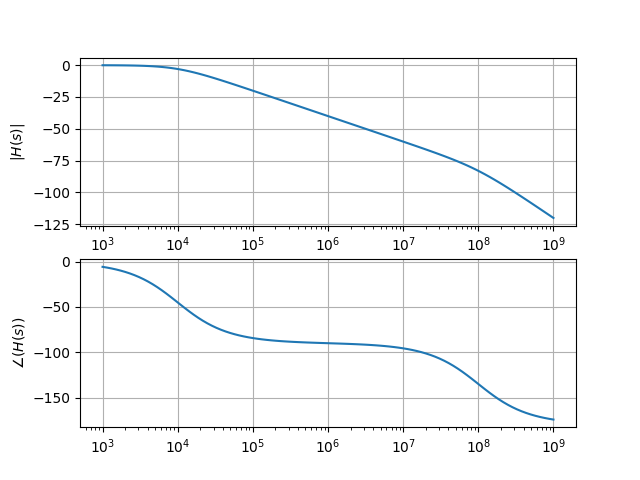
\includegraphics[scale=0.6]{Figure_4}
\centering
\caption{Bode Plots For RLC Low Pass Filter}
\label{fig:Coupled Oscillations}
\end{figure}

\clearpage

\subsection{Output Voltage}
We now plot the response of the low pass filter to the input:\newline
\begin{center}
$V_i(t) = (cos(10^3t) - cos(10^6t))u(t)$
\end{center}
for $0<t<30\mu s$ and $0<t<30ms$

\begin{lstlisting}
"""
This function returns Low pass filter 
response for given input and time period
"""
def RLC(t, R=100, L=1e-6, C=1e-6):
    H = sp.lti([1],[L*C,R*C,1])
    vi = np.multiply(np.cos(1000*t)-np.cos(1000000*t),np.heaviside(t,0.5))
    return sp.lsim(H,vi,t)

t = np.linspace(0,30*0.000001,10000)
_,y1,svec = RLC(t)
display_plot(5,t,y1,"Output Voltage for t<30$\mu s$", 't',r'$v_{o}(t)$')

t = np.linspace(0,30*0.001,10000)
_,y2,svec = RLC(t)
display_plot(6,t,y2,"Output Voltage for t<30ms",'t',r'$v_{o}(t)$')
\end{lstlisting}
\begin{figure}[h!]
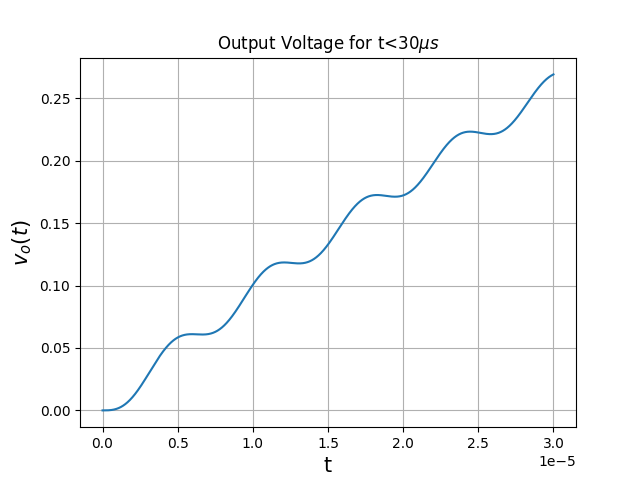
\includegraphics[scale=0.6]{Figure_5}
\centering
\caption{System response for $t<30\mu s$}
\label{fig:Coupled Oscillations}
\end{figure}
\begin{figure}[h!]
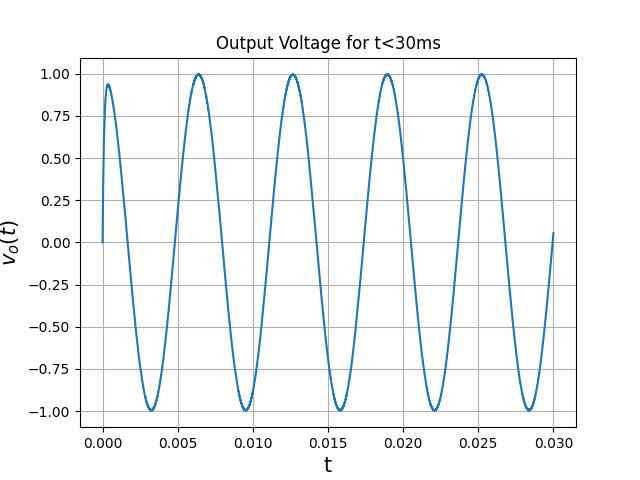
\includegraphics[scale=0.6]{Figure_6}
\centering
\caption{System response for $t<30ms$}
\label{fig:Coupled Oscillations}
\end{figure}


\section{Conclusion}
The scipy.signal library provides a useful toolkit of functions for circuit
analysis. The toolkit was used for the analysis of various LTI systems. Specifically we analyzed forced oscillatory systems, single spring, double mass systems and Electric filters

\begin{itemize}
\item We notice that the steady state response is a decaying sinusoidal function. Also, the decay is hard to observe when the decay constant = 0.5.

\item We notice that the time response of the system with much smaller decay constant is similar to that of the system with decay = 0.5, except with a
different amplitude. This is because the system takes longer to reach a steady
state.
Here, the amplitude (at moderate time) is much larger owing to a much
smaller decay.
	
\item The forced response of a simple spring body system was obtained
over various frequencies of the applied force, and highest amplitude was
observed at resonant frequency. Specifically, the natural frequency of the given system is w = 1.5 rad/s . Thus, as expected the maximum amplitude of oscillation is obtained when the frequency of f(t) is 1.5 rad/s , as a case of resonance.

\item A coupled spring problem was solved using
the sp.impulse function to obtain two sinusoids of the same frequency. We notice that the outputs of this system are 2 sinusoids of the same frequency, but
with different amplitude and phase.

\item A two-port network, functioning as a low-pass filter was analysed and the
output was obtained for a mixed frequency input. From the Bode plot of H(s), we notice that the system provides unity gain
for a low frequency of $10^3$
rad/s . Thus, the low frequency component is
more or less preserved in the output. However, the system dampens at high
frequency of $10^6$
rad/s. This is because of the inherent nature of the given circuit to act as a low pass filter.
\end{itemize}

\end{document}
